\newpage
\section{Problemas}

\question{
  Dados os vetores $\vec{u} = (2, -3, -1)$ e $\vec{v} = (1, -1, 4)$, calcular:
}
\begin{itemize}
  \item \subquestion{$2\vec{u} \cdot (-\vec{v})$}
    \answer{
      \begin{aligned}
        2\vec{u} &= (4, -6, -2) \\
        -\vec{v} &= (-1, 1, -4) \\
        2\vec{u} \cdot (-\vec{v}) &= 4\cdot-1 - 6\cdot(1) - 2\cdot(-4) \\
        &= -4 - 6 + 8 \\
        &= -2
      \end{aligned}
    }
  
  \item \subquestion{$(\vec{u} + 3\vec{v}) \cdot (\vec{v} - 2\vec{u})$}
    \answer{
      \begin{aligned}
        \vec{u} + 3\vec{v} &= (2 + 3(1), -3 + 3(-1), -1 + 3(4))  \\
        &= (5, -6, 11) \\
        \vec{v} - 2\vec{u} &= (1 - 2(2), -1 - 2(-3), 4 - 2(-1))  \\
        &= (-3, 5, 6) \\
        (\vec{u} + 3\vec{v}) \cdot (\vec{v} - 2\vec{u}) &=\\
        &= (5 * (-3), -6 * 5, 11 * 6) \\
        &= (-15, -30, 66) \\
        &= -15 - 30 + 66 = 21 \\
      \end{aligned}
    }
  \item \subquestion{$(\vec{u} + \vec{v}) \cdot (\vec{u} - \vec{v})$}
    \answer{
      \begin{aligned}
        \vec{u} + \vec{v} &= (3, -4, 3) \\
        \vec{u} - \vec{v} &= (1, -2, -5) \\
        (\vec{u}+\vec{v})\cdot(\vec{u}-\vec{v}) &= (3 * 1, -4 * (-2), 3 * (-5)) \\
        &= 3 + 8 - 15 = -4
      \end{aligned}
    }
  
  \item \subquestion{$(\vec{u} + \vec{v}) \cdot (\vec{v} - \vec{u})$}
    \answer{
      \begin{aligned}
        \vec{u} + \vec{v} &= (3, -4, 3) \\
        \vec{v} - \vec{u} &= (-1, 2, 3) \\
        (\vec{u} + \vec{v}) \cdot (\vec{v} - \vec{u})) &= (3 * (-1), -4 * 2, 3 * 3) \\
        &= -3 - 8 + 9 = -2
      \end{aligned}
    }
\end{itemize}

\newpage
\question{
  Sejam os vetores $\vec{u} = (2, a, -1)$, $\vec{v} = (3, 1, -2)$ e $\vec{w} =
  (2a - 1, -2, 4)$. Determinar $a$ de modo que:
  $\vec{u} \cdot \vec{v} = (\vec{u} + \vec{v}) \cdot (\vec{v} + \vec{w})$
}
\answer{
  \begin{aligned}
    \vec{u} \cdot \vec{v} &= (2 * 3) + (a * 1) + (-1 * (-2)) \\
                          &= (6) + (a) + (2) \\
                          &= 6 + a + 2 \\
                          &= 8 + a \\
    8 + a &= (\vec{u} + \vec{v}) \cdot (\vec{v} + \vec{w}) \\
          &= (5, a + 1, -3) \cdot (2a + 2, -1, 2) \\
          &= (5 * (2a + 2)) + ((a + 1) * -1) + (-3 * (2)) \\
          &= 10a + 10 - a - 1 + - 6 \\
    8 + a &= 9a + 3 \\
    9a - a &= 8 - 3 \\
        8a &= 5 \\
         a &= \frac{5}{8} \\
  \end{aligned}
}

\question{
  Dados os pontos $A(4, 0, -1)$, $B(2, -2, 1)$ e $C(1, 3, 2)$ e os vetores $\vec{u} = (2, 1, 1)$ e $\vec{v} = (-1, -2, 3)$, obter o vetor $\vec{x}$ tal que:
}
\begin{itemize}
\item \subquestion{$3\vec{x} + 2\vec{v} = \vec{x} + (\overrightarrow{AB} \cdot \vec{u}) \vec{v}$}
  \answer{
    \begin{aligned}
      \overrightarrow{AB} &= (-2, -2, 2) \\
      \overrightarrow{AB} \cdot \vec{u} &= (-2)(2) + (-2)(1) + (2)(1) = -4 - 2 + 2 = -4 \\
      3\vec{x} + 2\vec{v} &= \vec{x} + (-4)\vec{v} \\
      3\vec{x} + 2\vec{v} &= \vec{x} - 4\vec{v} \\
      2\vec{x} &= -6\vec{v} \\
      \vec{x} &= -3\vec{v} = -3(-1, -2, 3) = (3, 6, -9)
    \end{aligned}
  }
\item \subquestion{$(\overrightarrow{BC} \cdot \vec{v}) \vec{x} = (\vec{u} \cdot \vec{v}) \vec{v} - 3\vec{x}$}
  \answer{
    \begin{aligned}
      \overrightarrow{BC} &= (-1, 5, 1) \\
      \overrightarrow{BC} \cdot \vec{v} &= 1 - 10 + 3 = -6 \\
      \vec{u} \cdot \vec{v} &= -2 - 2 + 3 = -1 \\
      -6\vec{x} &= -\vec{v} - 3\vec{x} \\
      -3\vec{x} &= -\vec{v} \Rightarrow \vec{x} = \frac{1}{3} \vec{v} \\
      \vec{x} &= \left( -\frac{1}{3}, -\frac{2}{3}, 1 \right)
    \end{aligned}
  }
\end{itemize}

\newpage
\question{
  Determinar o vetor $\vec{v}$, paralelo ao vetor $\vec{u} = (2, -1, 3)$, tal
  que $\vec{v} \cdot \vec{u} = -42$.
}
\answer{
  \begin{aligned}
    \vec{v} &= k\vec{u} \\
    \vec{v} &= k(2, -1, 3) = (2k, -k, 3k) \\
    \vec{v} \cdot \vec{u} &= -42 \\
    (2k, -k, 3k) \cdot (2, -1, 3) &= -42 \\
    4k + k + 9k &= -42 \\
    14k &= -42 \\
    k &= -3
    \vec{v} = (-6, 3, -9)
  \end{aligned}
}

\question{
  Determinar o vetor $\vec{v}$ do espaço, sabendo que:
  \begin{itemize}
    \item $|\vec{v}| = 5$
    \item $\vec{v}$ é ortogonal ao eixo $Ox$
    \item $\vec{v} \cdot \vec{w} = 6$
    \item $\vec{w} = \vec{i} + 2\vec{j}$
  \end{itemize}
}
\answer{
  \begin{aligned}
    &\text{Como } \vec{v} \perp Ox \Rightarrow v_x = 0 \\
    &\vec{v} = (0, v_y, v_z)  \\
    &\vec{w} = (1, 2, 0) \\
    &\text{1. } |\vec{v}| = 5 \Rightarrow \sqrt{v_y^2 + v_z^2} = 5 \Rightarrow v_y^2 + v_z^2 = 25 \\
    &\text{2. } \vec{v} \cdot \vec{w} = 6 \Rightarrow (0)(1) + (v_y)(2) + (v_z)(0) = 6 \Rightarrow 2v_y = 6 \Rightarrow v_y = 3 \\
    &\text{Substituindo } v_y = 3 \text{ na 1ª equação:} \\
    &3^2 + v_z^2 = 25 \Rightarrow 9 + v_z^2 = 25 \Rightarrow v_z^2 = 16 \Rightarrow v_z = \pm 4 \\
    &\vec{v} = (0, 3, 4) \quad \text{e} \quad \vec{v} = (0, 3, -4) \\
  \end{aligned}
}

\question{
  Determinar o vetor $\vec{v}$, ortogonal ao eixo $Oy$, sabendo que:
  \begin{itemize}
    \item $\vec{v} \cdot \vec{v}_1 = 8$ com $\vec{v}_1 = (3, 1, -2)$
    \item $\vec{v} \cdot \vec{v}_2 = -3$ com $\vec{v}_2 = (-1, 1, 1)$
  \end{itemize}
}
\answer{
  \begin{aligned}
    &\text{Como } \vec{v} \perp Oy, \text{ então } \vec{v} = (x, 0, z) \\
    &\vec{v} \cdot \vec{v}_1 = 8 \Rightarrow (x, 0, z) \cdot (3, 1, -2) = 3x - 2z = 8 \\
    &\vec{v} \cdot \vec{v}_2 = -3 \Rightarrow (x, 0, z) \cdot (-1, 1, 1) = -x + z = -3 \\
    &\begin{cases}
    3x - 2z = 8 \\
    -x + z = -3 \\
    \end{cases} \\
    &\text{Multiplicando a segunda equação por 2: } -2x + 2z = -6 \\
    &\text{Somando com a primeira: } x = 2 \\
    &\text{Substituindo: } -2 + z = -3 \Rightarrow z = -1 \\
    &\vec{v} = (2, 0, -1)
  \end{aligned}
}

\newpage
\question{
  Dados os vetores $\vec{u} = (1, 2, -3)$, $\vec{v} = (2, 0, -1)$ e $\vec{w} = (3, 1, 0)$, determinar o vetor $\vec{x} = (x, y, z)$ tal que:
  \begin{itemize}
    \item $\vec{x} \cdot \vec{u} = -16$
    \item $\vec{x} \cdot \vec{v} = 0$
    \item $\vec{x} \cdot \vec{w} = 3$
  \end{itemize}
}
\answer{
  \begin{aligned}
    &\vec{x} = (x, y, z) \\
    &\vec{x} \cdot \vec{u} = -16 \Rightarrow x + 2y - 3z = -16 \quad \text{(1)} \\
    &\vec{x} \cdot \vec{v} = 0 \Rightarrow 2x - z = 0 \Rightarrow z = 2x \quad \text{(2)} \\
    &\vec{x} \cdot \vec{w} = 3 \Rightarrow 3x + y = 3 \Rightarrow y = 3 - 3x \quad \text{(3)} \\
    &\text{Substituindo (2) e (3) em (1):} \\
    &x + 2(3 - 3x) - 3(2x) = -16 \\
    &x + 6 - 6x - 6x = -16 \\
    &-11x + 6 = -16 \Rightarrow -11x = -22 \Rightarrow x = 2 \\
    &y = 3 - 3(2) = -3 \\
    &z = 2(2) = 4 \\
    &\vec{x} = (2, -3, 4)
  \end{aligned}
}

\question{
  Sabendo que $|\vec{u}| = 2$, $|\vec{v}| = 3$ e $\vec{u} \cdot \vec{v} = -1$,
  calcular:
}
\begin{itemize}
  \item \subquestion{$(\vec{u} - 3\vec{v}) \cdot \vec{u}$}
    \answer{
      \begin{aligned}
        (\vec{u} - 3\vec{v}) \cdot \vec{u} &= \vec{u} \cdot \vec{u} - 3\vec{v} \cdot \vec{u} \\
        &= |\vec{u}|^2 - 3(\vec{u} \cdot \vec{v}) \\
        &= 4 - 3(-1) \\
        &= 7 \\
      \end{aligned}
    }

  \item \subquestion{$(2\vec{v} - \vec{u}) \cdot (2\vec{v})$}
    \answer{
      \begin{aligned}
        (2\vec{v} - \vec{u}) \cdot (2\vec{v}) &= 4\vec{v} \cdot \vec{v} - 2\vec{u} \cdot \vec{v} \\
        &= 4|\vec{v}|^2 - 2(\vec{u} \cdot \vec{v}) \\
        &= 36 - 2(-1) \\
        &= 38 \\
      \end{aligned}
    }
  \item \subquestion{$(\vec{u} + \vec{v}) \cdot (\vec{v} - 4\vec{u})$}
    \answer{
      \begin{aligned}
        (\vec{u}+\vec{v})\cdot(\vec{v}-4\vec{u}) &= \vec{u}\cdot\vec{v} - 4\vec{u}\cdot\vec{u} + \vec{v}\cdot\vec{v} - 4\vec{v}\cdot\vec{u} \\
        &= (\vec{u}\cdot\vec{v}) - 4|\vec{u}|^2 + |\vec{v}|^2 - 4(\vec{u}\cdot\vec{v}) \\
        &= -1 - 16 + 9 + 4 \\
        &= -4 \\
      \end{aligned}
    }

  \newpage
  \item \subquestion{$(3\vec{u} + 4\vec{v}) \cdot (-2\vec{u} - 5\vec{v})$}
    \answer{
      \begin{aligned}
        (3\vec{u}+4\vec{v})\cdot(-2\vec{u}-5\vec{v}) &= 3\vec{u}\cdot(-2\vec{u}) + 3\vec{u}\cdot(-5\vec{v}) + 4\vec{v}\cdot(-2\vec{u}) + 4\vec{v}\cdot(-5\vec{v}) \\
        &= -6|\vec{u}|^2 - 15(\vec{u}\cdot\vec{v}) - 8(\vec{v}\cdot\vec{u}) - 20|\vec{v}|^2 \\
        &= -6(4) - 15(-1) - 8(-1) - 20(9) \\
        &= -24 + 15 + 8 - 180 \\
        &= -181 \\
      \end{aligned}
    }
\end{itemize}

\question{
  Calcular $\vec{u} \cdot \vec{v} + \vec{u} \cdot \vec{w} + \vec{v} \cdot
  \vec{w}$, sabendo que $\vec{u} + \vec{v} + \vec{w} = \vec{0}$, $|\vec{u}| =
  2$, $|\vec{v}| = 3$ e $|\vec{w}| = 5$.
}
\answer{
  \begin{aligned}
    &\text{Dado que } \vec{u} + \vec{v} + \vec{w} = \vec{0}, \text{ elevando ao quadrado ambos os lados:} \\
    &|\vec{u} + \vec{v} + \vec{w}|^2 = 0 \\
    &|\vec{u}|^2 + |\vec{v}|^2 + |\vec{w}|^2 + 2(\vec{u}\cdot\vec{v} + \vec{u}\cdot\vec{w} + \vec{v}\cdot\vec{w}) = 0 \\
    &2^2 + 3^2 + 5^2 + 2S = 0 \quad \text{(onde } S = \vec{u}\cdot\vec{v} + \vec{u}\cdot\vec{w} + \vec{v}\cdot\vec{w}) \\
    &4 + 9 + 25 + 2S = 0 \\
    &38 + 2S = 0 \\
    &2S = -38 \\
    &S = -19 \\
    &\vec{u} \cdot \vec{v} + \vec{u} \cdot \vec{w} + \vec{v} \cdot \vec{w} = -19
  \end{aligned}
}

\newpage
\question{
  Os pontos $A$, $B$ e $C$ são vértices de um triângulo equilátero cujo lado
  mede $20$ cm. Calcular $\overrightarrow{AB} \cdot \overrightarrow{AC}$ e
  $\overrightarrow{AB} \cdot \overrightarrow{CA}$.
}
\answer{
  \begin{minipage}[t]{0.48\textwidth}
    \begin{itemize}
      \item \subquestion{Cálculo de $\overrightarrow{AB} \cdot \overrightarrow{AC}$}
        \begin{aligned}
          &|\overrightarrow{AB}| = |\overrightarrow{AC}| = 20\, \text{cm} \\
          &\text{Ângulo entre } \overrightarrow{AB} \text{ e } \overrightarrow{AC} = 60^\circ \\
          &\overrightarrow{AB} \cdot \overrightarrow{AC} = |\overrightarrow{AB}||\overrightarrow{AC}|\cos(60^\circ) \\
          &= 20 \times 20 \times 0.5 = \boxed{200\, \text{cm}^2}
        \end{aligned}
    \end{itemize}
  \end{minipage}
  \hfill
  \begin{minipage}[t]{0.48\textwidth}
    \begin{itemize}
      \item \subquestion{Cálculo de $\overrightarrow{AB} \cdot \overrightarrow{CA}$}
        \begin{aligned}
          &\overrightarrow{CA} = -\overrightarrow{AC} \\
          &\overrightarrow{AB} \cdot \overrightarrow{CA} = \overrightarrow{AB} \cdot (-\overrightarrow{AC}) \\
          &= -(\overrightarrow{AB} \cdot \overrightarrow{AC}) \\
          &= -200\, \text{cm}^2 = \boxed{-200\, \text{cm}^2}
        \end{aligned}
    \end{itemize}
  \end{minipage}

  \begin{figure}[H]
    \centering
    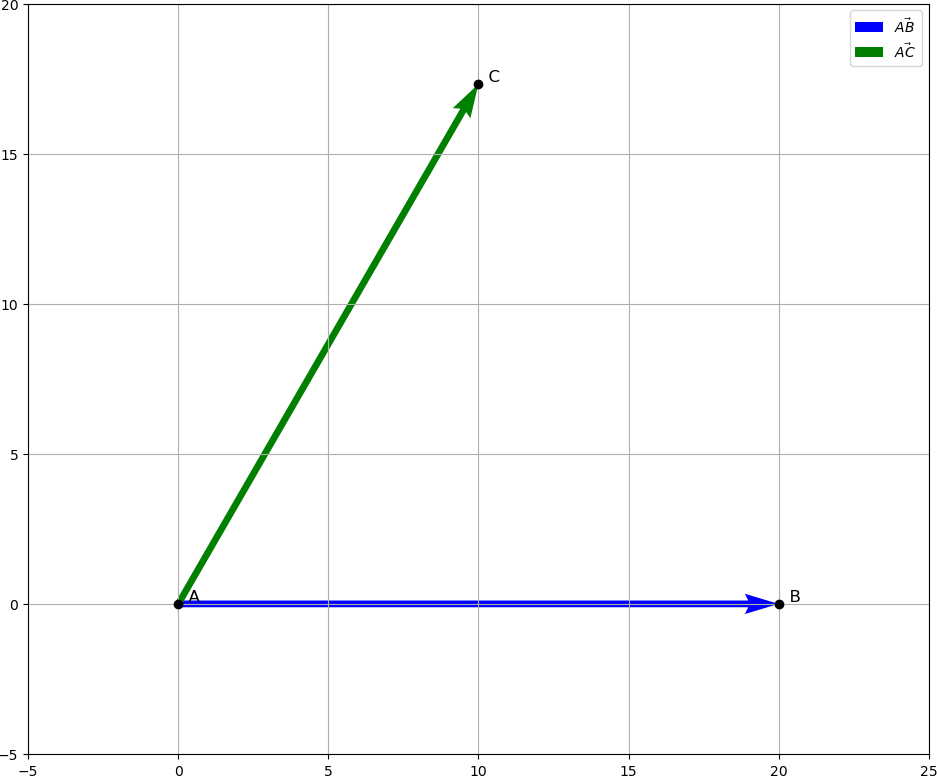
\includegraphics[width=0.8\textwidth]{./fig/q10.png}
    \caption{Triângulo equilátero ABC com lados de 20 cm, mostrando os vetores AB e AC com ângulo de 60° entre eles}
  \end{figure}
}
